\documentclass[12pt,letterpaper]{article}
\usepackage{fullpage}
\usepackage[top=2cm, bottom=4.5cm, left=2.5cm, right=2.5cm]{geometry}
\usepackage{amsmath,amsthm,amsfonts,amssymb,amscd}
% \usepackage{lastpage}
\usepackage{enumerate}
\usepackage{fancyhdr}
% \usepackage{mathrsfs}
\usepackage{xcolor}
% \usepackage{graphicx}
\usepackage{listings}
\usepackage{hyperref}

% Bayes Net Latex : https://github.com/jluttine/tikz-bayesnet
\usepackage{tikz}
\usetikzlibrary{bayesnet}

% define vector
\newcommand{\q}{\underline}

% define in-line code
\definecolor{codegray}{gray}{0.9}
\newcommand{\code}[1]{\colorbox{codegray}{\texttt{#1}}}

\hypersetup{%
  colorlinks=true,
  linkcolor=blue,
  linkbordercolor={0 0 1}
}

\renewcommand\lstlistingname{Snippet}
\renewcommand\lstlistlistingname{Snippet}
\def\lstlistingautorefname{Snippet.}

\lstdefinestyle{python}{
    language        = python,
    frame           = lines, 
    basicstyle      = \footnotesize,
    keywordstyle    = \color{violet},
    stringstyle     = \color{green},
    commentstyle    = \color{red}\ttfamily
}


\setlength{\parindent}{0.0in}
\setlength{\parskip}{0.05in}

% Edit these as appropriate
\newcommand\course{Phys 214}
\newcommand\NetIDa{Ming-Feng Ho}           % <-- NetID of person #1

\pagestyle{fancyplain}
\headheight 35pt
\lhead{\NetIDa}
\chead{\textbf{\Large Proposal Review}}
\rhead{\course \\ \today}
\lfoot{}
\cfoot{}
\rfoot{\small\thepage}
\headsep 1.5em

\begin{document}

\section*{Good proposal patterns}

Several interesting things happened during the discussion in the proposal panel. 
Besides I unfortunately forgot to prepare the presentation, 
I learned some patterns that people would generally think they are good proposals:

\begin{enumerate}
    \item \textbf{Observation proposal but includes simulations as a backup story}: 
    like the proposal of Gunn-Peterson trough. 
    It's a typical kind of proposal that people like. 
    Since it includes observation and simulation, 
    it's plausible both observers and simulators would vote for it.
    
    \item \textbf{Simulation proposal but includes achievable observations}: 
    e.g., neutrino mass proposal and lensing with the ray-tracing technique proposal. 
    People are generally less interested in those simulations which are untestable in the near future, 
    e.g., simulations from different dark matter candidates. 
    People expect simulations would improve our understanding of the observations. 
    So it's crucial that simulators should think about those observers when they are trying to write proposals. 
    Especially, if your simulations are not going to benefit observers' understandings to their data, 
    they will not give you money.

    \item \textbf{You already have something}: 
    proposals which already include some results are always preferred in our panel. 
    I feel this is a little bit controversial because how is that possible you already have results before you have funds to do the research you are going to do. 
    I also heard some people would use their past published results as their proposed research, 
    and use the new funding to do whatever they want to do.
\end{enumerate}

\section*{Things need to be avoided}

\begin{enumerate}
    \item \textbf{Avoid to use figures which are hard to explain}
    \item \textbf{Don't assume everyone knows what you are doing}
    \item \textbf{Write as easy as possible}
\end{enumerate}


\section*{Non-representative panel}

One essential thing people noticed during the discussion is that the reviewers (we) are not representative enough to reflect the actual proposal panel. 
For example, we have too many simulators, some earth scientists, and few observers.
The composition of our panel is heterogeneous and non-representative, so the voting result would certainly be biased.

My first thought is ``social science is hard''. 
The psychology survey data or political science voting forecast are always non-representative, I think. 
Calibrating the non-representative data and making on them is social scientists' bread and butter. 
 
I've read this paper\footnote{\url{https://www.microsoft.com/en-us/research/wp-content/uploads/2016/04/forecasting-with-nonrepresentative-polls.pdf}} before written by statistician Prof. Gelman.
By using hierarchical Bayesian modeling doing logistic regression, you can turn the non-representative survey to make robust predictions.
He called this method `` multilevel regression and poststratification (MRP)''. 
He used X-box to do the survey (, which for sure is non-representative because most of the players are male, ) and made an accurate forecast for the 2012 presidential election.

The concept of MRP is to combine hierarchical structure in Bayesian modeling with the poststratification.
The idea of poststratification is simple: we divide people into several cells based on their outcomes, e.g., genders, (theorists or observers or ...), ages, research interests (galaxy, AGN, exoplanet, IGM, ...), and so on. 
And to get an unbiased cell-level estimate, we simply do the average to get the mean value of the votings.
The poststratification part is to scale the value of voting to an existing representative group.
For example, we have five observers in our class, but, in reality, maybe the real panel for an observation proposal composited by 9/10 observers and 1/10 theorists.
So the poststratification procedure (if we assume we only have one outcome and one group in consideration) is to first take the average to the voting results within the cell (observer or theorist):

\begin{equation*}
    \begin{split}
        a_{\mathrm{theorist}}     &= (2 + 3 + 2 +2 +3 + 2) / 6 = 2.33\\
        a_{\mathrm{observer}}   &= (1 + 2 + 2 +1 +2) / 5 = 1.6
    \end{split}    
\end{equation*}

And then weighting the cell-level estimate to the representative group, 

\begin{equation*}
    a = 1 / 10 a_{\mathrm{theorist}} + 9 / 10 a_{\mathrm{observer}} = 1.67
\end{equation*}

Note that if we are not doing the poststratification, the result of voting we get is 2.0.
The assumption for taking average within the cell is that we assumed the sample is drawn randomly from the population.

The real life is not as simple as this example. 
To get a robust voting prediction, we have to consider all possible outcomes of the voters (us).
Moreover, there may have some hierarchical structure between outcomes. 
For example, the same outcomes (gender, (simulator or observer), research interests) may have different voting results based on which subgroup (astrophysics or earth science) the voter belongs to.
For instance, a researcher doing exoplanet in the astrophysics department may have a different voting result than an exoplaneter in the earth science department.

That's the reason why multilevel modeling would be helpful for poststratification. 
We could build a Bayes net (multilevel modeling) to do the parameter estimation on different levels.
The final step is just weighing the estimation based on the cell-level (or departmental-level) to an appropriate representative composition of the panel.

\begin{figure}
    \begin{center}
        % model_mrp_astro_earth.tex : the model for multilevel regression and poststratification
% in astro phys214 proposal panel
% using https://github.com/jluttine/tikz-bayesnet

% mrp model

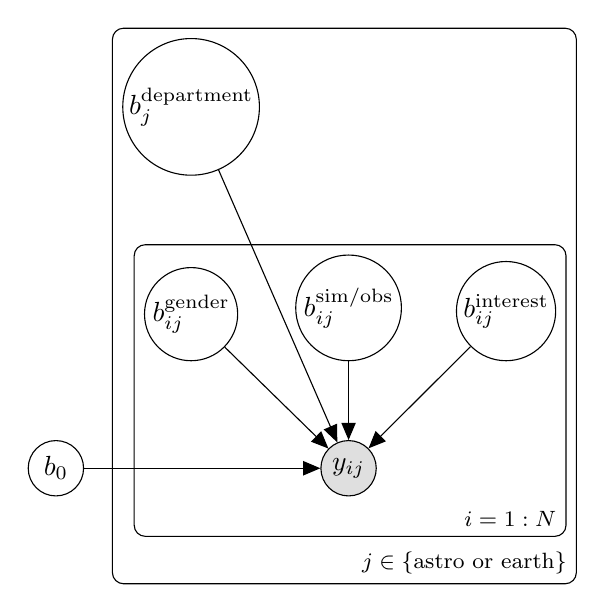
\begin{tikzpicture}

    % cell-level nodes
    \node[obs] (y) {$y_{ij}$};
    \node[latent, above=of y, xshift=-2cm] (b_gender)   {$b_{ij}^{\mathrm{gender}}$};
    \node[latent, above=of y, xshift=-0cm] (b_sim_obs)  {$b_{ij}^{\mathrm{sim/obs}}$};
    \node[latent, above=of y, xshift=2cm]  (b_interest) {$b_{ij}^{\mathrm{interest}}$};

    % group-level nodes
    \node[latent, above=of b_sim_obs, xshift=-2cm] (b_depart) {$b_{j}^{\mathrm{department}}$};

    \node[latent, left=of y, xshift=-2cm] (b_0) {$b_{0}$};
    
    % the connection
    \edge {b_gender, b_sim_obs, b_interest} {y};
    \edge {b_depart}                        {y};
    \edge {b_0}                             {y};

    % repetition plates
    \plate {cell} {(y)(b_gender)(b_sim_obs)(b_interest)} {$i = 1:N$};
    \plate {group} {(y)(b_gender)(b_sim_obs)(b_interest)(b_depart)(cell)} {$j \in \{\text{astro or earth}\}$};

\end{tikzpicture}        
    \end{center}
    \caption{A Bayes net designed for our proposal panel}
    \label{fig:bayes_net_mrp}
\end{figure}

See Fig~\ref{fig:bayes_net_mrp} for the Bayes net for my proposed model of voting in our panel.
The calculation of the probability would be, 

\begin{equation}
    \mathrm{Pr(y_{ij} = yes)} = \mathrm{logit^{-1}}(
        b_0 + b_j^{\mathrm{department}} + b_{ij}^{\mathrm{gender}}
        + b_{ij}^{\mathrm{sim/obs}} + b_{ij}^{\mathrm{interest}}
    ).
\end{equation}

Assume $b_{ij}^{\mathrm{outcomes}}$ are randomly sampled from a prior distribution,
and then fit the logistic regression model to the data.

Finally, poststratificate the $\mathrm{Pr(y_{ij} = yes)}$ probabilities using the 
weighting estimated from the representative population.
I would be interested in testing the model if I have the voting result and the composition of a real proposal panel.

\section*{Comments from class}

\begin{enumerate}
    \item Able to explain the negative results
    \item Give enough background
    \item Connected theory with observations
    \item Abstract like the first date
    \item Stay with the experienced one
    \item Having someone not in your field to read your draft
    \item Avoid arrogant
    \item Don't use jargon
    \item Don't use figures
\end{enumerate}

\end{document}
